\documentclass[twoside]{book}

% Packages required by doxygen
\usepackage{fixltx2e}
\usepackage{calc}
\usepackage{doxygen}
\usepackage[export]{adjustbox} % also loads graphicx
\usepackage{graphicx}
\usepackage[utf8]{inputenc}
\usepackage{makeidx}
\usepackage{multicol}
\usepackage{multirow}
\PassOptionsToPackage{warn}{textcomp}
\usepackage{textcomp}
\usepackage[nointegrals]{wasysym}
\usepackage[table]{xcolor}

% NLS support packages
\usepackage[french]{babel}

% Font selection
\usepackage[T1]{fontenc}
\usepackage[scaled=.90]{helvet}
\usepackage{courier}
\usepackage{amssymb}
\usepackage{sectsty}
\renewcommand{\familydefault}{\sfdefault}
\allsectionsfont{%
  \fontseries{bc}\selectfont%
  \color{darkgray}%
}
\renewcommand{\DoxyLabelFont}{%
  \fontseries{bc}\selectfont%
  \color{darkgray}%
}
\newcommand{\+}{\discretionary{\mbox{\scriptsize$\hookleftarrow$}}{}{}}

% Page & text layout
\usepackage{geometry}
\geometry{%
  a4paper,%
  top=2.5cm,%
  bottom=2.5cm,%
  left=2.5cm,%
  right=2.5cm%
}
\tolerance=750
\hfuzz=15pt
\hbadness=750
\setlength{\emergencystretch}{15pt}
\setlength{\parindent}{0cm}
\setlength{\parskip}{3ex plus 2ex minus 2ex}
\makeatletter
\renewcommand{\paragraph}{%
  \@startsection{paragraph}{4}{0ex}{-1.0ex}{1.0ex}{%
    \normalfont\normalsize\bfseries\SS@parafont%
  }%
}
\renewcommand{\subparagraph}{%
  \@startsection{subparagraph}{5}{0ex}{-1.0ex}{1.0ex}{%
    \normalfont\normalsize\bfseries\SS@subparafont%
  }%
}
\makeatother

% Headers & footers
\usepackage{fancyhdr}
\pagestyle{fancyplain}
\fancyhead[LE]{\fancyplain{}{\bfseries\thepage}}
\fancyhead[CE]{\fancyplain{}{}}
\fancyhead[RE]{\fancyplain{}{\bfseries\leftmark}}
\fancyhead[LO]{\fancyplain{}{\bfseries\rightmark}}
\fancyhead[CO]{\fancyplain{}{}}
\fancyhead[RO]{\fancyplain{}{\bfseries\thepage}}
\fancyfoot[LE]{\fancyplain{}{}}
\fancyfoot[CE]{\fancyplain{}{}}
\fancyfoot[RE]{\fancyplain{}{\bfseries\scriptsize Généré par Doxygen }}
\fancyfoot[LO]{\fancyplain{}{\bfseries\scriptsize Généré par Doxygen }}
\fancyfoot[CO]{\fancyplain{}{}}
\fancyfoot[RO]{\fancyplain{}{}}
\renewcommand{\footrulewidth}{0.4pt}
\renewcommand{\chaptermark}[1]{%
  \markboth{#1}{}%
}
\renewcommand{\sectionmark}[1]{%
  \markright{\thesection\ #1}%
}

% Indices & bibliography
\usepackage{natbib}
\usepackage[titles]{tocloft}
\setcounter{tocdepth}{3}
\setcounter{secnumdepth}{5}
\makeindex

% Hyperlinks (required, but should be loaded last)
\usepackage{ifpdf}
\ifpdf
  \usepackage[pdftex,pagebackref=true]{hyperref}
\else
  \usepackage[ps2pdf,pagebackref=true]{hyperref}
\fi
\hypersetup{%
  colorlinks=true,%
  linkcolor=blue,%
  citecolor=blue,%
  unicode%
}

% Custom commands
\newcommand{\clearemptydoublepage}{%
  \newpage{\pagestyle{empty}\cleardoublepage}%
}

\usepackage{caption}
\captionsetup{labelsep=space,justification=centering,font={bf},singlelinecheck=off,skip=4pt,position=top}

%===== C O N T E N T S =====

\begin{document}

% Titlepage & ToC
\hypersetup{pageanchor=false,
             bookmarksnumbered=true,
             pdfencoding=unicode
            }
\pagenumbering{alph}
\begin{titlepage}
\vspace*{7cm}
\begin{center}%
{\Large T\+P3 Simulation }\\
\vspace*{1cm}
{\large Généré par Doxygen 1.8.13}\\
\end{center}
\end{titlepage}
\clearemptydoublepage
\pagenumbering{roman}
\tableofcontents
\clearemptydoublepage
\pagenumbering{arabic}
\hypersetup{pageanchor=true}

%--- Begin generated contents ---
\chapter{Index des fichiers}
\section{Liste des fichiers}
Liste de tous les fichiers avec une brève description \+:\begin{DoxyCompactList}
\item\contentsline{section}{\hyperlink{main_8c}{main.\+c} \\*Implémentations et tests des fonctions créees pour le TP n°3 de Simulation }{\pageref{main_8c}}{}
\end{DoxyCompactList}

\chapter{Documentation des fichiers}
\hypertarget{main_8c}{}\section{Référence du fichier main.\+c}
\label{main_8c}\index{main.\+c@{main.\+c}}


Implémentations et tests des fonctions créees pour le TP n°3 de Simulation.  


{\ttfamily \#include $<$stdio.\+h$>$}\newline
{\ttfamily \#include $<$math.\+h$>$}\newline
{\ttfamily \#include \char`\"{}mt19937ar.\+h\char`\"{}}\newline
Graphe des dépendances par inclusion de main.\+c\+:\nopagebreak
\begin{figure}[H]
\begin{center}
\leavevmode
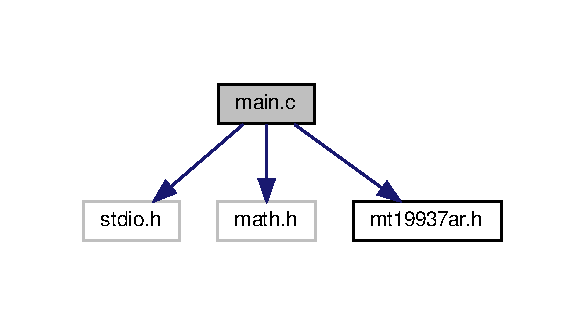
\includegraphics[width=281pt]{main_8c__incl}
\end{center}
\end{figure}
\subsection*{Fonctions}
\begin{DoxyCompactItemize}
\item 
double \hyperlink{main_8c_a003a6336831c638f315bd28d987cd6ae}{get\+\_\+quantil} (int ind)
\begin{DoxyCompactList}\small\item\em Fonction qui permet d\textquotesingle{}obtenir les quantils à partir du tableau t\+\_\+values. \end{DoxyCompactList}\item 
double \hyperlink{main_8c_ac29441dc1e67ba3bdf8ff2fd6e80b590}{approx\+\_\+pi} (int number)
\begin{DoxyCompactList}\small\item\em Fonction permettant d\textquotesingle{}approximer le nombre PI. \end{DoxyCompactList}\item 
double \hyperlink{main_8c_a9dc62e75fa2e58d2ebad4921c30c1b1f}{mean\+\_\+pi} (int n, double $\ast$pis, int number)
\begin{DoxyCompactList}\small\item\em Fonction utilisant plusieurs fois la fonction \hyperlink{main_8c_ac29441dc1e67ba3bdf8ff2fd6e80b590}{approx\+\_\+pi()} afin d\textquotesingle{}en faire une moyenne. \end{DoxyCompactList}\item 
double \hyperlink{main_8c_a9b205782961c1259d3a9f39dffa995bb}{variance} (int n, double $\ast$pis, double mean)
\begin{DoxyCompactList}\small\item\em Fonction calculant une estimation sans biais de la variance d\textquotesingle{}un tableau (en l\textquotesingle{}occurence de PI) \end{DoxyCompactList}\item 
void \hyperlink{main_8c_ad89cd222c09aca0d2a6f5309eaf1eb1f}{confidences\+\_\+intervals\+\_\+95} (int n, double mean, double v, double $\ast$b\+\_\+inf, double $\ast$b\+\_\+sup)
\begin{DoxyCompactList}\small\item\em Fonction qui calcule les intervalles de confiances à 95\%. \end{DoxyCompactList}\item 
void \hyperlink{main_8c_a7633736232754889999b8605b977795e}{gen\+\_\+lapins} (int mois, unsigned long $\ast$population)
\begin{DoxyCompactList}\small\item\em Fonction générant une population de lapins (Suite de Fibonacci) \end{DoxyCompactList}\item 
int \hyperlink{main_8c_ae66f6b31b5ad750f1fe042a706a4e3d4}{main} ()
\end{DoxyCompactItemize}
\subsection*{Variables}
\begin{DoxyCompactItemize}
\item 
const double \hyperlink{main_8c_a001b1492c3bdf863e991eb1ffb0f0c3c}{t\+\_\+values} \mbox{[}$\,$\mbox{]}
\begin{DoxyCompactList}\small\item\em Tableau des quantiles. \end{DoxyCompactList}\end{DoxyCompactItemize}


\subsection{Description détaillée}
Implémentations et tests des fonctions créees pour le TP n°3 de Simulation. 

\begin{DoxyAuthor}{Auteur}
Mathieu Arquilliere (\href{mailto:mathieu.arquilliere@etu.uca.fr}{\tt mathieu.\+arquilliere@etu.\+uca.\+fr}) 
\end{DoxyAuthor}
\begin{DoxyVersion}{Version}
1 
\end{DoxyVersion}
\begin{DoxyDate}{Date}
2019-\/10-\/15
\end{DoxyDate}
\begin{DoxyCopyright}{Copyright}
Copyright (c) 2019 
\end{DoxyCopyright}


\subsection{Documentation des fonctions}
\mbox{\Hypertarget{main_8c_ac29441dc1e67ba3bdf8ff2fd6e80b590}\label{main_8c_ac29441dc1e67ba3bdf8ff2fd6e80b590}} 
\index{main.\+c@{main.\+c}!approx\+\_\+pi@{approx\+\_\+pi}}
\index{approx\+\_\+pi@{approx\+\_\+pi}!main.\+c@{main.\+c}}
\subsubsection{\texorpdfstring{approx\+\_\+pi()}{approx\_pi()}}
{\footnotesize\ttfamily double approx\+\_\+pi (\begin{DoxyParamCaption}\item[{int}]{number }\end{DoxyParamCaption})}



Fonction permettant d\textquotesingle{}approximer le nombre PI. 


\begin{DoxyParams}{Paramètres}
{\em number} & Nombre d\textquotesingle{}itérations sur la méthode Monte-\/\+Carlo -\/$>$ précision du retour \\
\hline
\end{DoxyParams}
\begin{DoxyReturn}{Renvoie}
double Approximation du nombre PI 
\end{DoxyReturn}


Définition à la ligne 104 du fichier main.\+c.

Voici le graphe des appelants de cette fonction \+:
\nopagebreak
\begin{figure}[H]
\begin{center}
\leavevmode
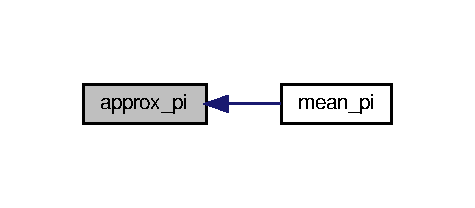
\includegraphics[width=228pt]{main_8c_ac29441dc1e67ba3bdf8ff2fd6e80b590_icgraph}
\end{center}
\end{figure}
\mbox{\Hypertarget{main_8c_ad89cd222c09aca0d2a6f5309eaf1eb1f}\label{main_8c_ad89cd222c09aca0d2a6f5309eaf1eb1f}} 
\index{main.\+c@{main.\+c}!confidences\+\_\+intervals\+\_\+95@{confidences\+\_\+intervals\+\_\+95}}
\index{confidences\+\_\+intervals\+\_\+95@{confidences\+\_\+intervals\+\_\+95}!main.\+c@{main.\+c}}
\subsubsection{\texorpdfstring{confidences\+\_\+intervals\+\_\+95()}{confidences\_intervals\_95()}}
{\footnotesize\ttfamily void confidences\+\_\+intervals\+\_\+95 (\begin{DoxyParamCaption}\item[{int}]{n,  }\item[{double}]{mean,  }\item[{double}]{v,  }\item[{double $\ast$}]{b\+\_\+inf,  }\item[{double $\ast$}]{b\+\_\+sup }\end{DoxyParamCaption})}



Fonction qui calcule les intervalles de confiances à 95\%. 


\begin{DoxyParams}[1]{Paramètres}
\mbox{\tt in}  & {\em n} & nombre d\textquotesingle{}occurences \\
\hline
\mbox{\tt in}  & {\em mean} & moyenne \\
\hline
\mbox{\tt in}  & {\em v} & variance \\
\hline
\mbox{\tt out}  & {\em b\+\_\+inf} & borne inferieure de l\textquotesingle{}intervalle de confiance \\
\hline
\mbox{\tt out}  & {\em b\+\_\+sup} & borne supérieur de l\textquotesingle{}intervalle de confiance \\
\hline
\end{DoxyParams}


Définition à la ligne 177 du fichier main.\+c.

Voici le graphe d\textquotesingle{}appel pour cette fonction \+:
\nopagebreak
\begin{figure}[H]
\begin{center}
\leavevmode
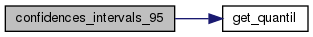
\includegraphics[width=307pt]{main_8c_ad89cd222c09aca0d2a6f5309eaf1eb1f_cgraph}
\end{center}
\end{figure}
Voici le graphe des appelants de cette fonction \+:

%--- End generated contents ---

% Index
\backmatter
\newpage
\phantomsection
\clearemptydoublepage
\addcontentsline{toc}{chapter}{Index}
\printindex

\end{document}
